\documentclass[10pt]{article}
% \usepackage[letterpaper,text={6.5in,8.7in},centering]{geometry}
\usepackage{curves}
\usepackage{epic,eepic,color}
%\usepackage[usenames,dvipsnames,svgnames,table]{xcolor}
% \usepackage{amssymb,amsmath,times,subfigure,graphicx,theorem}
\usepackage{alltt}
%\usepackage{warmread}
%\usepackage[all,import]{xy}
%\usepackage{eepic}
\usepackage{my_packages}
\usepackage{lastpage}
\usepackage{fancyhdr}
\pagestyle{fancy}
\cfoot{\thepage\ of \pageref{LastPage}}
\renewcommand{\headrulewidth}{0pt}
\usepackage{tikz_packages}
\renewcommand{\baselinestretch}{1.2}
\date{}

\renewcommand{\thesubsection}{\arabic{subsection}. }
\renewcommand{\thesubsubsection}{\arabic{subsection}.\arabic{subsubsection} }

\theoremstyle{definition}
\newtheorem{prob}{Problem}[section]
%\renewcommand{\theprob}{\arabic{section}.\arabic{prob}}
\renewcommand{\theprob}{\arabic{prob}}

\newenvironment{subprob}%
{\renewcommand{\theenumi}{\alph{enumi}}\renewcommand{\labelenumi}{(\theenumi)}\begin{enumerate}}%
{\end{enumerate}}%


%1: Explain the Newtonian gravitational force and gravitational potential between particles
%2: Analyze the characteristics of circular, elliptic, parabolic and hyperbolic orbits in a two-dimensional plane
%3: Apply numerical/analytical techniques to propogate orbits
%4: Describe the geometry of an orbit in a three-dimensional space from orbital elements


\begin{document}


\setcounter{page}{0}

\vspace*{1cm}

\centerline{\LARGE{ MAE3145: Final Exam}}
\vspace*{0.5cm}
\centerline{\Large \SI{2458052.1979}{\julianday}}%\\%\vspace*{0.5cm}

\vspace*{6cm}

\centerline{
\begin{tabular}{lll}
\hspace*{5cm}, & \hspace*{5cm}. & \hspace*{4cm}\\\hline
Last Name & First Name & Student ID
\end{tabular}}

\vspace*{6cm}

\centerline{
\begin{tabular}{|c|c|c|c|c|}\hline
Prob. 1 & Prob. 2 & Prob. 3 & Prob. 4 & Total \\
(18) & (40) & (22) & (20) & (100)\\ \hline
\hspace*{2.2cm} & \hspace*{2.2cm} & \hspace*{2.2cm} & \hspace*{2.2cm} & \hspace*{2.2cm}\\
                & & & & \\
                & & & & \\
\hline
\end{tabular}}

\clearpage\newpage
% \renewcommand{\theprob}{\arabic{prob} \textit{(15pt)}}

\begin{prob}
    Your spacecraft is currently in a \underline{circular} orbit about Planet X with \( \Omega = \SI{90}{\degree}\) and \( i = \SI{30}{\degree} \) relative to an inertial reference frame defined by \( \hat{x}, \hat{y}, \hat{z} \).
    At the \underline{descending node}, the following maneuver is implemented:
    \begin{align*}
        \bar \Delta v = \frac{1}{\sqrt{2}} \hat{V} - \hat{C} + \sqrt{\frac{3}{2}} \hat{N} \si{\kilo\meter\per\second} .
    \end{align*}

    Express the \( \Delta \bar v \) in terms of :
    \begin{subprob}
        \item Inertial reference frame: \( \hat x, \hat y, \hat z\)
        \item \(\norm{\Delta \bar v}, \alpha, \beta\) relative to the \( \hat V, \hat N, \hat C\) reference frame
    \end{subprob}
\end{prob}
\clearpage\newpage
\null\newpage
\null\newpage

\begin{prob}
    Assume that a spacecraft is moving in an orbit about the Earth characterized by \( e = 0.5\) and \( a = 4 R_\oplus\).
    To meet some scientific objective, an \underline{in-plane} maneuver is planned to adjust the orbit.
    The new orbit has exactly the same eccentricity and semi-major axis but periapsis will advance by \SI{90}{\degree}.
    \begin{subprob}
        \item The maneuver can be implemented at one of two values of true anomaly. 
            Determine these two options.
        \item Assume that the maneuver will be implemented at \( \theta = \SI{45}{\degree}\).
            Determine the required maneuver in terms of \( \norm{\Delta \bar v} \) and \(\alpha\).
    \end{subprob}
    \vspace*{9cm} 
    \begin{figure*}[hb]
        \centering
        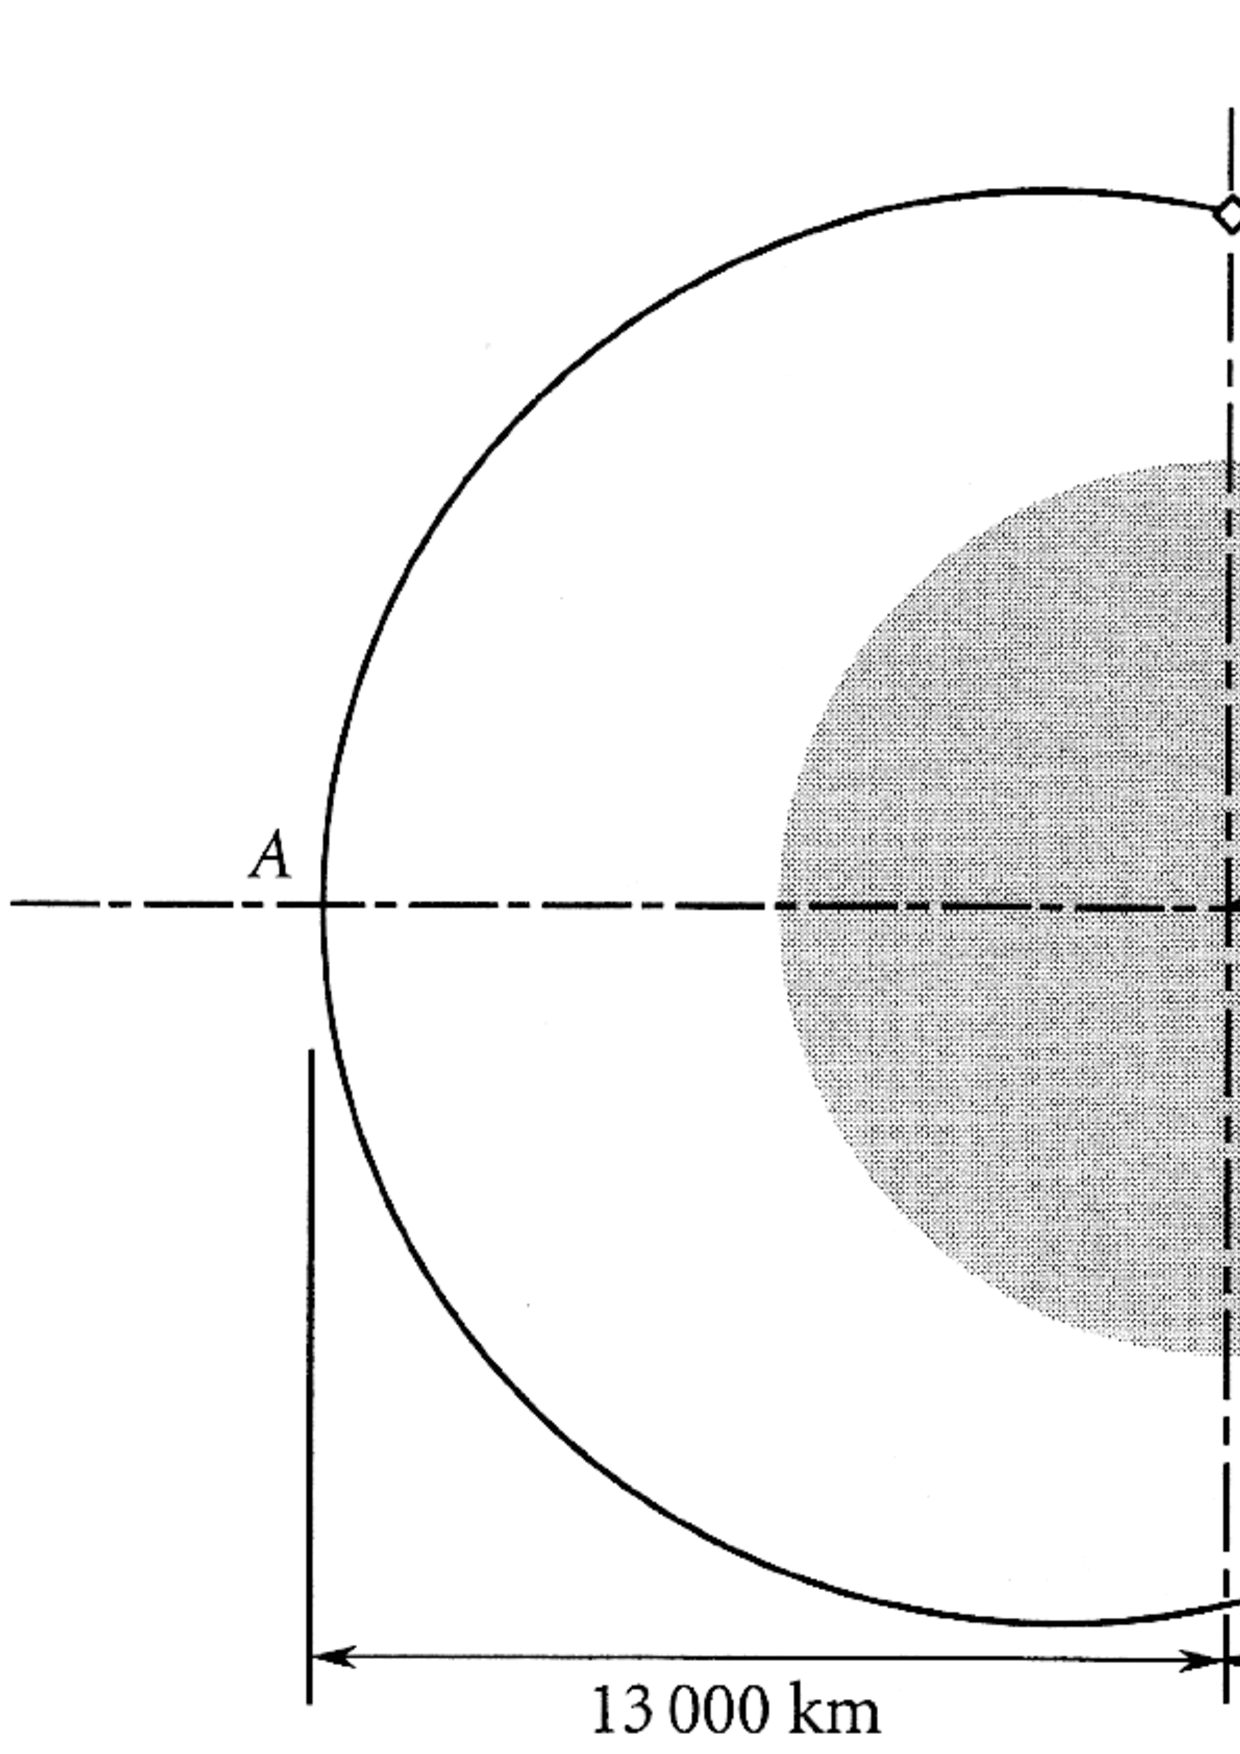
\includegraphics[width=\textwidth]{prob2.png}
    \end{figure*}
\end{prob}
\clearpage\newpage
\null\newpage
\null\newpage

\begin{prob}
    A vehicle is in a circular orbit about the Earth with radius \( r_1 = 6 R_\oplus\).
    A Hohmann transfer is employed to shift to a smaller, coplanar  circular orbit of \( r_2 = 2 R_\oplus\).
    \begin{subprob}
        \item Determine \( \Delta \bar v_{\text{total}}\) and the time of flight.
        \item Indicate if each manuever increase or decreases the instaneous speed.
    \end{subprob}
\end{prob}

\clearpage\newpage
\null\newpage
\null\newpage

\begin{prob}
    Develop an algorithm to determine the \textbf{PERIOD OF THE PHASING ORBIT} for a non-coplanar rendezvous problem to deploy a satellite from an inclined circular low Earth orbit to a higher, circular equatorial orbit at the \textbf{first opportunity}.
    The first  few steps have been outlined for you; complete the remaining algorithm.

\noindent\textbf{GIVEN:} \\
        Interceptor satellite COEs: \( a_{int}, i, \Omega, \theta\)\\
        Target satellite COEs: \( a_{tgt}, \theta\)

\noindent\textbf{FIND:} \\
Period of phasing orbit : \( \mathbb{P}_{\text{phasing}}\)

\begin{enumerate}
\item Calculate the angular speed ( mean motion) for both interceptor and target.
    \begin{align*}
        \omega_{int} = \sqrt{\frac{\mu}{a_{int}^3}} \qquad \omega_{tgt} = \sqrt{\frac{\mu}{a_{tgt}^3}}
    \end{align*}

\item Calculate the TOF for the Hohmann transfer (complete the equation below).
    \vspace*{2cm}
\item Calculate ...
\end{enumerate}
\end{prob}
\clearpage\newpage
\null\newpage
\null\newpage

\begin{prob}
    A radar tracking site is located at the following location: (assume a perfectly spherical Earth)
    \begin{itemize}
        \item Latitude: \SI{90}{\degree} North
        \item Altitude: \SI{0}{\kilo\meter}
        \item Local Sidereal Time: \SI{180}{\degree}
    \end{itemize}

    A satellite is in a circular polar orbit with \( a = \SI{9020.5}{\kilo\meter}, \Omega = \SI{90}{\degree}, \theta = \SI{45}{\degree}\).

    Determine the following:
    \begin{subprob}
    \item \textbf{Range-Vector} from the site to the satellite in the Geocentric Inertial Reference frame.
    \item \textbf{Elevation angle} and \textbf{Range} from the site to the satellite
    \end{subprob}
\end{prob}

\clearpage\newpage
\null\newpage
\null\newpage

\begin{prob}
    Draw a picture to explain why Greenwich Sidereal Time is approximately \SI{100}{\degree} at \num{0000} UTC on 1 January each year.
    Recall that the Winter Solstice is in the third week of December annually.
\end{prob}

\begin{prob}
    Given the total energy of a circular orbit, show that the orbital speed is constant and given by \( v_{circ} = \sqrt{\frac{\mu}{r}}\).
\end{prob}

\begin{prob}
    The Molniya orbit is a highly eccentric orbit specifically designed such that the spacecraft spends the majority of time in the vicinity of apogee.
    How would you determine the velocity of the Molniya orbit  at \underline{perigee}?
    Assume you are given the semi-major axis, \( a \), and eccentricity, \( e\).
    Express your solution in terms of \( a \) and \( e\).

    \begin{subprob}
        \item Determine the inclination required such that the argument of perigee remains constant?
        \item At this inclination what is the rate of right ascnension of the ascending node?
    \end{subprob}
\end{prob}

\clearpage\newpage
\null\newpage
\null\newpage
\begin{prob}
    To prepare for anti-satellite avoidance, US Space Command will require every satellite operator to generate a plot of total \( \Delta V \) versus time of flight (TOF) for their satellite to increase its altitude by \SI{25}{\kilo\meter}. 
    Provide an algorithm to generate this plot assuming that the satellites are initially in a circular orbit and the final orbit is circular and in the same inclination as the initial orbit. 
    Furthermore, assume that the first maneuver will be a tangential burn, while the second maneuver will be non-tangential ( a so called \textbf{One Tangent Burn}).

    \begin{subprob}
    \item Write your algorithm.
        Please write neatly and legibly.
        Furthermore, your algorithm should be in a logical sequence. 

        \textbf{GIVEN:} \( r_i\) (initial radius of circular orbit) and \( \Delta \nu\) (change in true true anomaly along the transfer orbit) from \SIrange{0}{180}{\degree}.

        \textbf{FIND:} Total \( \Delta V\) and TOF (time of flight)

        \vspace{0.5\textheight}
    \item Draw a vector diagram showing all three velocity vecotr involved in the second burn and label them correctly.
        Include the change in flight path angle \( \Delta \gamma \) and firing angle \( \alpha \).
    \end{subprob} 
\end{prob}    

\clearpage\newpage
\null\newpage
\null\newpage

\begin{prob}
    Your first job involves a boss who is aware of the SEZ frame but claims ``it doesn't make any sense''.
    Your boss would instead like to use the \textbf{North West Zenith} reference frame because it makes more sense.

    \begin{subprob}
    \item Determine the rotation matrices to transform a vector from the \textbf{North West Zenith} reference frame to the \textbf{Earth Centered Inertial} reference frame.
    \item From a site located at \SI{30}{\degree} North latitude and \SI{90}{\degree} West longitude, the range vector to a satellite is :
        \begin{align*}
            \bar \rho_{NWZ} = - 7000 \hat N - 500 \hat W + 500 \hat Z \si{\kilo\meter}
        \end{align*}
        at \( GST = 0600\) hours.
        What is the \( \hat k = \hat z \) component of this vector, \( \bar \rho_{ECI}\), in the \textbf{Earth Centered Inertial} reference frame?
    \end{subprob}
\end{prob}
\end{document}
